 %!TEX root = ../lectures_olympics.tex
 
 \chapter{电磁感应}
 \begin{wrapfigure}{o}{7cm}
 \includegraphics[width=7cm]{images/mag-3.pdf} 
 \caption{法拉弟和它的电磁感应实验}
 \end{wrapfigure}
前面我们已经看到运动的电荷,也就是电流可以产生磁场,在磁场中的电流,或运动的带电粒子可以受到磁场力的作用。
在此基础上人们自然会猜测,既然运动的电荷能够产生磁场,那么磁场也可能会产生电流。
在经过一系列的探索之后,磁场能够产生电效应的现象终于由法国科学家法拉弟({\it M. Faraday})所证实:在磁场当中运动的导体棒能够产生回路当中的电流,这一现象被称为{\heiti 电磁感应}(electromagnetic induction)。
导体内的自由电子在磁场当中运动时会受到洛伦兹力作用,当它们受到的洛伦兹力有沿导线方向的分量时,在导线内部就有了搬动电子的力,宏观上看就相当于有一个电动势,以这种方式形成的电动势被称做{\heiti 感应电动势}(electromotive force)。
进一步的实验和理论发展也表明,不仅是磁场当中运动的导线的情况下有可能产生感应电动势,对于固定的导线,当磁场的大小或方向发生变化时也有可能产生感应电动势,为了和运动导体棒的情况进行区分,运动导体产生的电动势又被称做{\heiti 动生电动势}(motional emf),而由磁场的变化产生的电动势则被称为{\heiti 感生电动势}(transformer emf),它们都是由于导体回路当中磁场的变化而产生的。
利用电磁感应现象可以将机械能转化为电能,彻底使人类社会进入电气化时代。

 
 
 
 \section{电磁感应定律}
和电场类似,当空间当中存在有磁场时,同样可以定义通过一给定曲面的磁感线的通量,称为{\heiti 磁通量}(magnetic flux)。
对于如图\ref{fig: 磁通量的定义}所示的匀强磁场$B$,它与面积为$S$的平面法线方向的夹角为$\theta$,那么穿过该平面区域的磁通量被定义为
\begin{equation}
\Phi = \vec{B}\cdot\vec{S} = BS\cos\theta.
\end{equation}
对于空间当中任意的磁场分布以及一般的曲面,穿过该曲面的磁通量被定义为穿过每个面积元$\Delta S$的磁通量的代数和:
\begin{equation}
\Phi = \int_S \vec{B}\cdot d\vec{S},
\end{equation}
当曲面或磁场分布有某种对称性的话,确定穿过曲面的磁通量实际上并不需要计算面积分。
\begin{figure}[hbtp]
\centering
\includegraphics[width = 0.6\textwidth]{images/mag-1.pdf}
\caption{(a)通过平面的匀强磁场,(b)一般的情况需要计算面积分}\label{fig: 磁通量的定义}
\end{figure}

当穿过一个闭合的导体回路的磁通量发生变化时,将在该回路当中产生感应电动势。
实验表明感应电动势的大小正比于穿过该曲面磁通量随时间的变化率,其方向由{\heiti 楞次定律}(Lenz's Law)给出:感应电流的磁场总要阻碍引起感应电流的磁通量的变化,用数学表示即
\begin{equation}\label{eqn: 电磁感应-电磁感应定律}
\mathcal{E} = -\frac{d\Phi}{dt}.
\end{equation}
当回路中没有电源时,所有的电动势全部来自于电场力的作功,这时对于一个闭合回路电动势可以记作电场沿着回路的线积分,此时电磁感应定律还可以写为
\begin{equation}
\oint_L \vec{E}\cdot d\vec{l} = -\frac{d}{dt}\int_S \vec{B}\cdot d\vec{S},
\end{equation}
其中$L$代表任意一个闭合回路,而$S$则是任意一个以此回路为边界的曲面,上式对于任意的回路和曲面均成立。


\subsection{动生电动势}
匀强磁场当中匀速运动的导体棒可以展示最简单的电磁感应现象,如图所示在垂直于磁感应强度为$B$的磁场方向有两个平等的导轨,导轨上有一根可以自由运动的,长度为$l$的导体棒。
当导体棒在某一时刻运动速度为$v$时,整个导体回路当中的磁通量会随着导体回路形状的变化而变化。
由电磁感应定律\ref{eqn: 电磁感应-电磁感应定律}可知,这种情况下磁通量随时间的变化率
\begin{equation}
\frac{d\Phi}{dt} = \frac{d}{dt}(BS) = B\frac{dS}{dt} = Blv
\end{equation}
结合楞次定律可知这时回路中的感应电动势
\begin{equation}\label{eqn: 电磁感应-blv}
\mathcal{E} = -\frac{d\Phi}{dt} = -Blv,
\end{equation}
方向沿着图中的逆时针方向,此时如果回路中的电阻为$R$时,将会有大小为
\begin{equation}
I=\frac{Blv}{R}
\end{equation}
的感应电流。



\begin{example}
动生电动势的本质是导体内的自由电子在磁场中运动会受到的洛伦兹力,洛伦兹力是电子运动的趋动力。
试证明垂直于匀强磁场以速度为$v$运动的导体棒上的感应电动势\ref{eqn: 电磁感应-blv}与从微观上电子沿回路运动时洛伦兹力的功一致。
\tagged{student}{\vspace*{4cm}}
\begin{taggedblock}{teacher}
\newline
解析:电子只有在运动的导轨上时才会受到洛伦兹力的作用,当导轨运动速度为$v$时电子受到的洛伦兹力
\[f=eBv\]
沿着长度为$l$的运动导轨方向运动洛伦兹力作功
\[W = fl =eBvl\]
这样电子从棒的一端运动到另一端单位电荷的功自然就是$Blv$,与动生电动势一致。
\end{taggedblock}
\end{example}

\begin{example}
如图所示有垂直于纸面向外、强度为$B$的匀强磁场 ,一导体杆可在轨道上摩擦地滑动,为了使导体棒做速度为$v$的匀速直线运动,需要有外力$F$维持。
试证明外力的功率与消耗在电阻$R$上的电功率相等,忽略电路其它部分的电阻。
\begin{flushright}
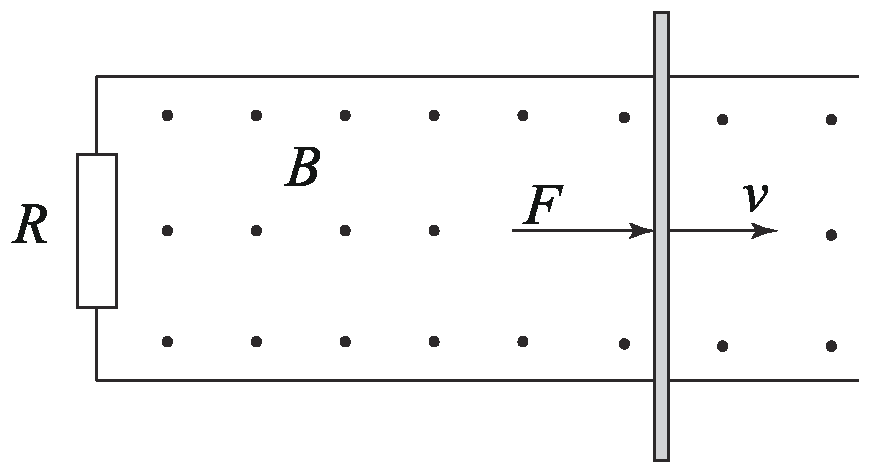
\includegraphics[width = 0.4\textwidth]{images/mag-14.pdf} 
\end{flushright}
\tagged{student}{\vspace*{1cm}}
\begin{taggedblock}{teacher}
\noindent
解析:回路电阻为$R$时,感应电流的大小
\[I = \frac{Blv}{R},\]
这样运动的导线受到的安培力
\[F = IBl = \frac{B^2l^2v}{R}\]
为了使它匀速运动,需要有相同大小的力作用在上面,这样外力的功率自然就是
\[P_F=Fv=\frac{B^2l^2v^2}{R}\]
忽略其它部分电阻时,消耗在电阻上的电功率
\[P_e = UI =Blv \frac{Blv}{R}=\frac{B^2l^2v^2}{R}\]
很明显与外力的功率相等。
\end{taggedblock}
\end{example}




\begin{example}
若无外力作用,求如图所示电路中初速度为$v_0$的导体棒速度随时间的变化规律;到完全静止之前所走过的总路程以及整个过程中流过电阻的总电量。
已知导体棒的质量为$m$,与导轨的摩擦忽略不计,导轨无限长且电阻可以忽略。
\begin{flushright}
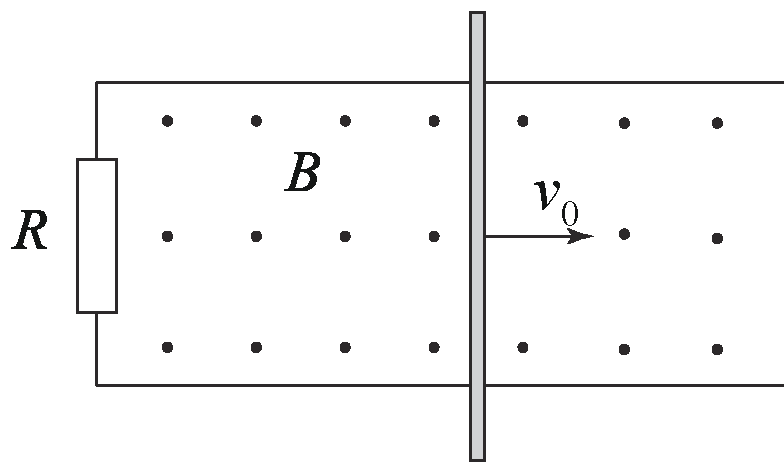
\includegraphics[width = 0.3\textwidth]{images/mag-15.pdf} 
\end{flushright}
\tagged{student}{\vspace*{1cm}}
\begin{taggedblock}{teacher}
\noindent
解析:当导轨运动速度为$v$时,回路中的电流$I=\frac{Blv}{R}$,这样作用在运动导轨上的安培力大小为
\[F = \frac{B^2l^2}{R}v\]
方向与运动速度方向相反,这样导轨的运动可以看成是在正比于速度的阻力下的减速运动,其运动方程为
\[
m\frac{dv}{dt}=-\frac{B^2l^2}{R}v
\]
已知初速度为$v_0$,此后的运动很容易解出:
\[
v(t)=v_0e^{-\frac{B^2l^2}{mR}t}
\]
\end{taggedblock}
\end{example}




%%%%%%%%%%%%%%%%%
\begin{example}

某同学用电荷量计(能测出一段时间内通过导体横截面的电荷量)测量地磁场强度,完成了如下实验:如图,将面积为$S$,电阻为$R$的矩形导线框$abcd$沿图示方位水平放置于地面上某处,将其从图示位置绕东西轴转$180^\circ$,测得通过线框的电荷量为$Q_1$;将其从图示位置绕东西轴转$90^\circ$,测得通过线框的电荷量为$Q_2$。
该处地磁场的磁感应强度大小应为
\[
A. \frac{R}{S}\sqrt{\frac{Q_1^2}{4}+Q_2^2},\qquad B. \frac{R}{S}\sqrt{Q_1^2+Q_2^2}\qquad C. \frac{R}{S}\sqrt{\frac{Q_1^2}{4}+Q_1Q_2+Q_2^2}\qquad \frac{R}{S}\sqrt{Q_1^2+Q_1Q_2+Q_2^2}
\]
\begin{flushright}
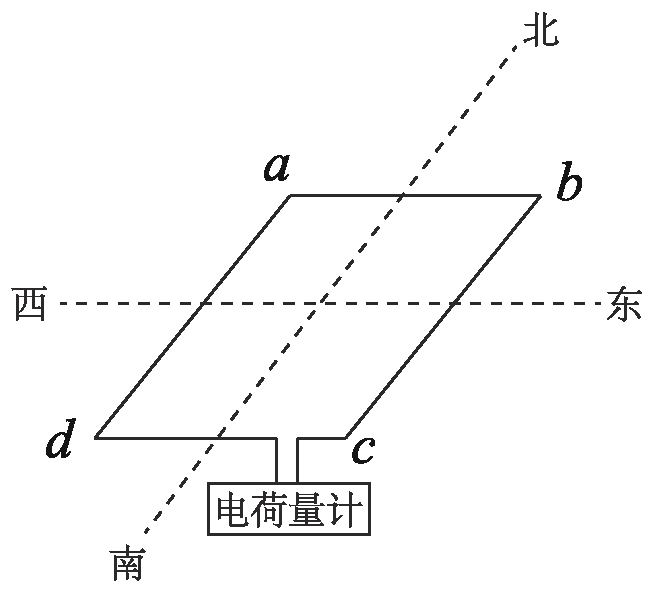
\includegraphics[width = 0.3\textwidth]{images/mag-32.pdf} 
\end{flushright}
\tagged{student}{\vspace*{1cm}}
\begin{taggedblock}{teacher}
\noindent
解析:C
\end{taggedblock}
\end{example}
%%%%%%%%%%%%%%%%%%%%%%


%%%%%%%%%%%%%%%%%%%%%%%%%%%%%%%%%%
\begin{example}
如图所示,已知电源电动势为$\mathcal{E}$,内阻为$r$,跟电阻$R$连接后与足够长的间距为$L$的平行金属导轨连接,$ab$为金属棒,它能在导轨上自由滑动。
金属棒和导轨电阻可忽略不计,彼此间滑动摩擦力$F$是个恒量,匀强磁场$B$的方向已在图中标出。

1. 求开关$S$接通后金属棒$ab$的极限速度$v_{m}$;

2. 如果这一极限速度$v_{m}$是磁场$B$的函数,问$B$多大时,$v_{m}$有最大值?这时对应的电流多大?

3. 如果$r>R$,$ab$棒速度为$v_p$值时,电池有最大输出功率$P_{max}$,求$P_{max}$与$v_p$的表达式。
\begin{flushright}
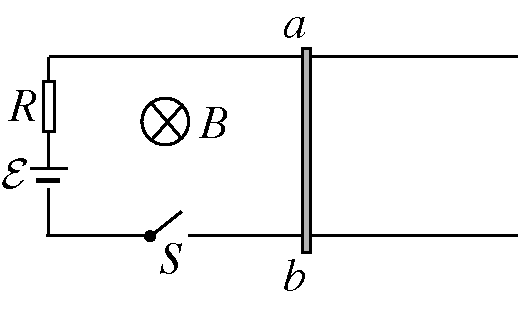
\includegraphics[width=0.4\textwidth]{images/mag-25.pdf}
\end{flushright}
\tagged{student}{\vspace*{4cm}}
\begin{taggedblock}{teacher}
\noindent
解析:1. $v_m=\frac{\varepsilon}{Bl}-\frac{F(r+R)}{B^2l^2}$
\\2.$B=\frac{2F(r+R)}{\varepsilon l}$,$I=\frac{\varepsilon}{2(R+r)}$
\\3.$P_max=(\frac{\varepsilon-Blv_p}{R+r})^2*R$
\end{taggedblock}
\end{example}
%%%%%%%%%%%%%%%%%%%%%%%%%%

\begin{example}
匀强磁场中有一个面积为$S$的导线圈在外力作用下作匀速圆周运动,角速度为$\omega$,
导线的另一端接有一个定值电阻$R$,求回路中电流随时间关系$I(t)$。
\begin{flushright}
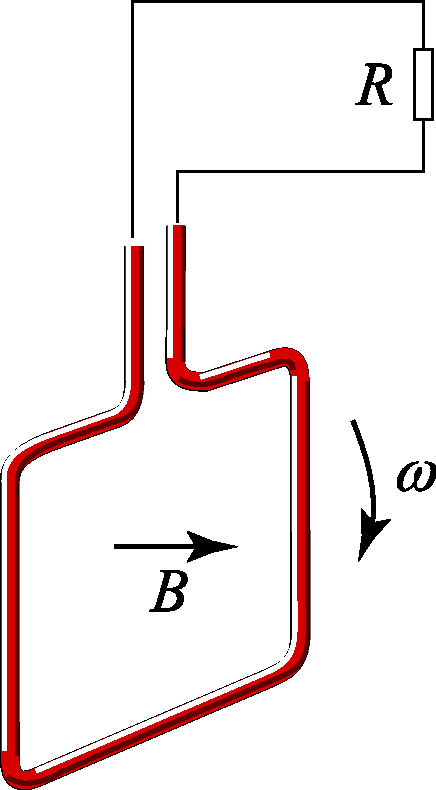
\includegraphics[width = 0.2\textwidth]{images/mag-16.pdf} 
\end{flushright}

\tagged{student}{\vspace*{0cm}}
\begin{taggedblock}{teacher}
\noindent
解析:穿过导线的磁通量$\Phi = BS\cos\omega t$,根据电磁感应定律电动势
\[
\mathcal{E} = -\frac{d\Phi}{dt} = BS\omega\sin\omega t
\]
这样线路中的电流
\[
I(t) = \mathcal{E}/R = \frac{\omega BS}{R}\sin\omega t
\]
\end{taggedblock}
\end{example}



%%%%%%%%%%%%%%%%%
\begin{example}
如图所示的“日”字型线框,每一段长度均为$l=0.1\unit{m}$,ab、cf、de段的电阻为$3\Omega$,cd、ef段电阻$1.5\Omega$,bc、af两段电阻可忽略。
整个线框处在与线框平面垂直的匀强磁场$B=1\unit{T}$中,其边界与ab边平行。
如果以$v=24\unit{m/s}$的速度将线圈匀速拉出磁场区,求此过程拉力做的功。
\begin{flushright}
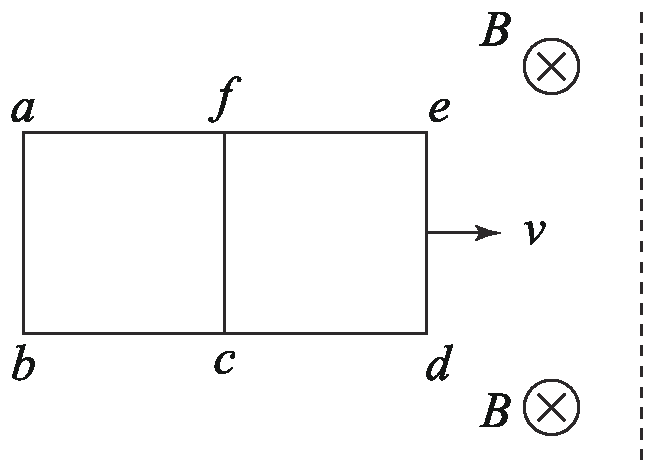
\includegraphics[width = 0.4\textwidth]{images/mag-43.pdf} 
\end{flushright}

\tagged{student}{\vspace*{4cm}}
\begin{taggedblock}{teacher}
\noindent
解析:0.008J
\end{taggedblock}
\end{example}
%%%%%%%%%%%%%%%%%%%%%%

\begin{example}
如图所示,在无限长直线电流旁边,有边长为$a $和$b $的矩形线框,线框绕它的一条长边(平行于直线电流)为固定轴,以角速度$\omega$旋转。
已知直线电流为$I$,它与转轴的距离为$(a+c)$,若从线框平面与直线电流在同一平面内时开始计时,试问经多少时间线框中的感应电动势第一次达最大值,该值为多大?
\begin{flushright}
\includegraphics[width = 0.3\textwidth]{images/mag-17.pdf} 
\end{flushright}
\tagged{student}{\vspace*{4cm}}
\begin{taggedblock}{teacher}
\noindent
解析:$\cos \omega t=\frac{2a(a+c)}{a^2+(a+c)^2},\varepsilon=\frac{\omega \mu a^2I}{2\pi}\frac{a+c}{c(2a-c)}$
\end{taggedblock}
\end{example}


%%%%%%%%%%%%%%%%%
\begin{example}

如图所示,一绝缘容器内部为立方体空腔,其长和宽分别为$a$和$b$,厚度为$d$,其两侧等高处装有两根与大气相通的玻璃管(可用来测量液体两侧的压强差)。
容器内装满密度为$\rho$的导电液体,容器上下两端装有铂电极$A $和$C$,这样就构成了一个液体电阻。
该液体电阻置于一方向与容器的厚度方向平行的均匀恒定的磁感应强度为$B$ 的磁场中,并通过开关$K $接在一电动势为$\mathcal{E}$、内阻为$r$的电池的两端。
闭合开关,若稳定时两侧玻璃管中液面的高度差为$h$,求导电液体的电导率$\sigma$,已知重力加速度大小为$g$。
\begin{flushright}
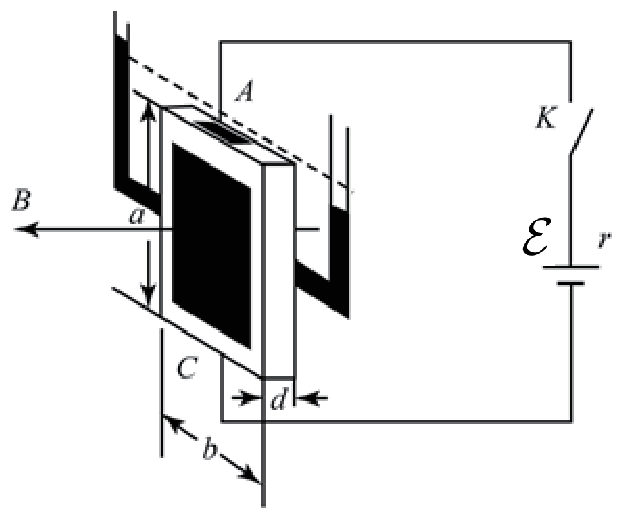
\includegraphics[width = 0.3\textwidth]{images/mag-29.pdf} 
\end{flushright}

\tagged{student}{\vspace*{4cm}}
\begin{taggedblock}{teacher}
\noindent
解析:$\sigma=\frac{\rho gha}{b(B\varepsilon-r\rho ghd)}$
\end{taggedblock}
\end{example}
%%%%%%%%%%%%%%%%%%%%%%

\subsection{感生电动势}
电磁感应定律告诉我们,不仅导线在磁场中运动会产生感应电动势,在回路形状不变但磁场大小发生改变时同样有可能产生感应电动势。
简单起见假设有如图所示的磁场,在任一时刻磁场的大小和方向均与位置无关,但磁场的大小与时间有关系$B=B(t)$,磁场当中有面积为$S$的导体回路,这时同样会产生感应电动势。
根据感应电动势的数学描述\ref{eqn: 电磁感应-电磁感应定律}可知此时回路中的感应电动势为
\begin{equation}
\mathcal{E} = -\frac{d\Phi}{dt} = -S\frac{dB}{dt},
\end{equation}
方向同样可以由楞次定律所决定,这就是所谓的{\heiti 感生电动势}最简单的情况。

这时导体回路中趋动自由电子运动的力并不是动生电动势时的洛伦兹力,而是由于磁场的变化在空间中产生感应电场的结果。
这是我们第一次碰到电场和磁场的相互转化的例子,如图\ref{fig: 涡旋电场}所示的当空间当中一点上的磁感应强度随时间而变时,会在它周围产生一个小的电场,其方向与磁感应强度变化的方向相反,大小正比于磁感应强度的变化率,因为它总是具有围绕着磁感线的环形结构,所以这种感生电场就被称作{\heiti 涡旋电场}(eddy electric field)。
当一个闭合回路内部磁场发生变化时,回路内的感生电动势的起源为所有涡旋电场对带电粒子作功的总和。
\begin{figure}[hbtp]
\centering
\includegraphics[width=0.7\textwidth]{images/mag-2.pdf}
\caption{(a)空间每点上磁感应强度变化时产生的涡旋电场,(b)磁场中导体回路中的感生电动势为其内部涡旋电场的总和}\label{fig: 涡旋电场}
\end{figure}



\begin{example}
一个半径为$r$的圆形导线环处于磁感应强度为$B_0$的匀强磁场当中,它的总电阻为$R$,磁场方向与导线平面法线方向的夹角为$\theta$,当移去磁场之后由于电磁感应导线内将出现感应电流,求从移去磁场开始直到形成最终稳定状态的过程中通过导体某一横截面的总电量。
\tagged{student}{\vspace*{4cm}}
\begin{taggedblock}{teacher}
\newline
解析:开始时刻穿过导线的磁通量$\Phi = B_0\pi r^2\cos\theta$,在移去磁场的过程中根据电磁感应定律
\[
\mathcal{E} = -\frac{\Delta \Phi}{\Delta t} = IR,
\]
将上式变形可得
\[
\Delta \Phi = IR\Delta t = R\Delta Q,
\]
对时间积分并化简可得
\[
Q = \sum \Delta Q = \Delta \Phi/R = \frac{B_0\pi r^2\cos\theta}{R}
\]
\end{taggedblock}
\end{example}




%%%%%%%%%%%%%%%%%
\begin{example}

小磁铁在铝制空心杆中运动(无裂缝、有裂缝、有交错矩形裂孔),先落地的是哪一个。
\tagged{student}{\vspace*{4cm}}
\begin{taggedblock}{teacher}
\newline
解析:有裂缝的那一个,因为椤次定律,磁铁运动产生的感应电流会阻碍其原有的运动,而这三种情况下有裂缝的那个金属管无法构成回路,所以几乎不会产生感应电流,因此它不受额外力的作用,所以先落地。
\end{taggedblock}
\end{example}
%%%%%%%%%%%%%%%%%%%%%%



%%%%%%%%%%%%%%%%%
\begin{example}
如图,电阻为$R$的长直螺线管,其两端通过电阻可忽略的导线相连接。
一个质量为$m$的小条形磁铁从静止开始落入其中,经过一段距离后以速度$v$ 做匀速运动。
假设小磁铁在下落过程中始终沿螺线管的轴线运动且无翻转。
 
⑴ 定性分析说明:小磁铁的磁性越强,最后匀速运动的速度就越小;

⑵ 小磁铁做匀速运动时在回路中产生的感应电动势约为多少?

\begin{flushright}
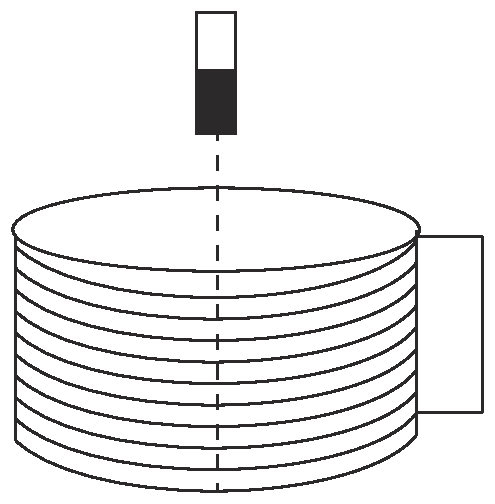
\includegraphics[width = 0.3\textwidth]{images/mag-34.pdf} 
\end{flushright}


\tagged{student}{\vspace*{3cm}}
\begin{taggedblock}{teacher}
\noindent
解析:1.根据楞次定律,小磁铁的磁性越强,通过导线环的磁通量的变化率越大,因此下落过程中在导线环中产生的感应电流越大,此感应电流产生的磁场也越强,从而对小磁铁的阻碍也越大,小磁铁向下运动的加速度越小,因此其极限速度就越小。
\\2.$E=mgRv$
\end{taggedblock}
\end{example}
%%%%%%%%%%%%%%%%%%%%%%

%%%%%%%%%%%%%%%%%
\begin{example}
在一半径为$R$的无限长密绕螺线管中有一均匀磁场,磁感应强度随时间线性变化(即$\frac{\Delta B}{\Delta t} = k$。
现用单位长度电阻为$r $的导体线弯成半径为$a$的圆环,并把此环与螺线管同心放置。

1. 求圆环中电流(考虑$a>R $和$a<R $两种情况);

2. 圆环上处于同一直径上两点$AC$之间的电压$U_{AC}$是多少。



\tagged{student}{\vspace*{4cm}}
\begin{taggedblock}{teacher}
\noindent
解析:1.$a>R:I=\frac{kR^2}{2r}\frac{1}{a};a<R:I=\frac{ka}{2r}$
\\2. 为0
\end{taggedblock}
\end{example}
%%%%%%%%%%%%%%%%%%%%%%


%%%%%%%%%%%%%%%%%
\begin{example}
电子感应加速器利用变化的磁场来加速电子。
电子绕平均半径为$R$的环形轨道(轨道位于真空管道内)运动,磁感应强度方向与环形轨道平面垂直。电子被感应电场加速,感应电场的方向与环形轨道相切,电子电荷量为$e$。

1. 设电子做圆周运动的环形轨道上的磁感应强度大小的增加率为$\frac{\Delta B}{\Delta t}$,求在环形轨道切线方向感应电场作用在电子上的力;

2. 设环形轨道平面上的平均磁感应强度大小的增加率为$\frac{\Delta \overline{B}}{\Delta t}$,试导出在环形轨道切线方向感应电场作用在电子上的力与$\frac{\Delta \overline{B}}{\Delta t}$的关系;

3. 为了使电子在不断增强的磁场中沿着半径不变的圆轨道加速运,求$\frac{\Delta B}{\Delta t}$和$\frac{\Delta \overline{B}}{\Delta t}$之间必须满足的定量关系。

\begin{flushright}
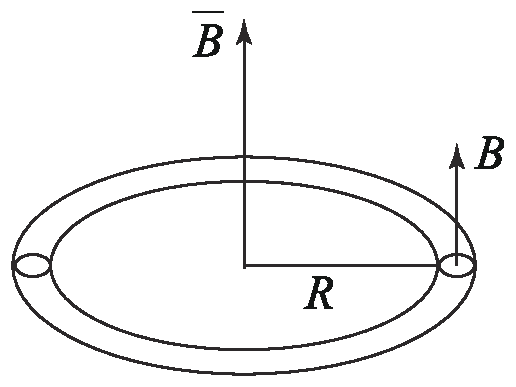
\includegraphics[width = 0.4\textwidth]{images/mag-33.pdf} 
\end{flushright}
\tagged{student}{\vspace*{3cm}}
\begin{taggedblock}{teacher}
\noindent
解析:当磁场增加时,电子会受到更多的向心力,为了维持在圆轨道上的运动电子必须加速,电子沿运动方向的加速满足牛顿第二定律$F\Delta t = m\Delta v$,而当$B$发生变化时需要的速度增加量满足$m\Delta v = eR\Delta B$,两式联立可得电子需要的径向力
\[
F = eR\frac{\Delta B}{\Delta t}.
\]
电子的径向力由变化磁场引起的涡旋电场给出,涡旋电场满足电磁感应定律
\[
2\pi R E = \pi R^2\frac{\Delta \overline{B}}{\Delta t},\qquad F = eE = \frac{1}{2}eR\frac{\Delta \overline{B}}{\Delta t},
\]
为了让加速器正常工作,要求两者保持时刻同步
\[
\frac{\Delta B}{\Delta t}=\frac{1}{2}\frac{\Delta \overline{B}}{\Delta t}.
\]
\end{taggedblock}
\end{example}
%%%%%%%%%%%%%%%%%%%%%%

%%%%%%%%%%%%%%%%%
\begin{example}

如图,半径为$R$的圆柱形区域内有匀强磁场,磁场方向垂直纸面指向纸外,磁感应强度$B$随时间均匀变化,变化率$\frac{\Delta B}{\Delta t} = K$($K$ 为一正值常量),圆柱形区外空间没有磁场,沿图中$AC$弦的方向画一直线,并向外延长,弦$AC$与半径$OA$的夹角$\alpha = \pi/4$。
直线上有一任意点,设该点与$A$点的距离为$x$,求从$A$沿直线到该点的电动势的大小。
\begin{flushright}
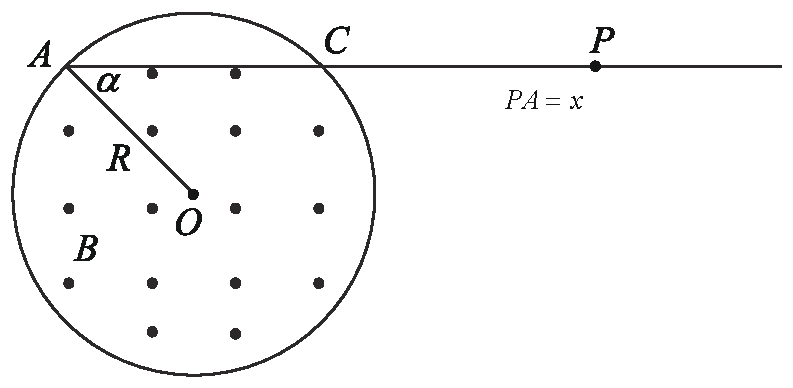
\includegraphics[width = 0.5\textwidth]{images/mag-23.pdf} 
\end{flushright}
\tagged{student}{\vspace*{4cm}}
\begin{taggedblock}{teacher}
\noindent
解析:1.任意点在磁场区域内:$E_{AP}=\frac{kR}{2\sqrt{2}}x$
\\2.任意点在磁场区域外:$E_{AQ}=\frac{kR^2}{2}(1+\arctan\frac{x-\sqrt{2}R}{x})$
\end{taggedblock}
\end{example}
%%%%%%%%%%%%%%%%%%%%%%


%%%%%%%%%%%%%%%%%
\begin{example}
一个用绝缘材料制成的扁平薄圆环,其内、外半径分别为$R_1$、$R_2$,厚度可以忽略.
两个表面都带有电荷,电荷面密度$\sigma$随离开环心距离$r$变化的规律均为$ \sigma(r) = \frac{\sigma_0}{r^2}$,$\sigma_0$为已知常量。
薄圆环绕通过环心垂直环面的轴以大小不变的角加速度$\beta$减速转动,$t = 0$时刻的角速度为$\omega_0$。
将一半径为$r$($r<<R_1$)、电阻为$R$并与薄圆环共面的导线圆环与薄圆环同心放置。

试求在薄圆环减速运动过程中导线圆环中的张力$F$与时间$t$的关系。

提示:半径为$r$、通有电流$I$的圆线圈(环形电流),在圆心处产生的磁感应强度为$B = \frac{\mu_0I}{2r}$。
\begin{flushright}
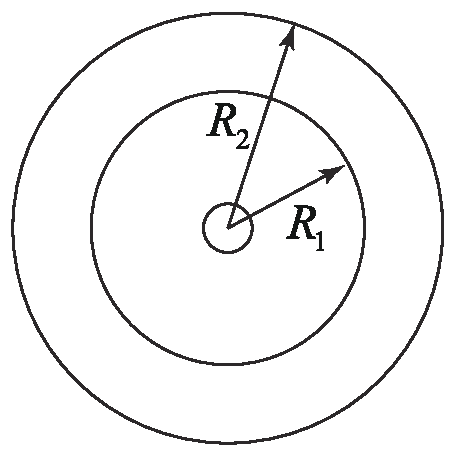
\includegraphics[width = 0.3\textwidth]{images/mag-35.pdf} 
\end{flushright}


\tagged{student}{\vspace*{4cm}}
\begin{taggedblock}{teacher}
\noindent
解析:积分得圆心磁场强度$B=\frac{\mu_0 \sigma_0\omega d}{2}(\frac{1}{R_1}-\frac{1}{R_2})$,注意r处的电流可以表示为$Q(r)*\omega$
\\薄圆环有电流I:$R*I=\varepsilon=\frac{\Delta B}{\Delta t}*S=\frac{\mu_0 \sigma_0\beta d}{2}(\frac{1}{R_1}-\frac{1}{R_2})*\pi r^2$
\\张力为F,$2*F\sin\frac{\theta}{2}=BIr*\Delta\theta$
\\解出:$F=\frac{\mu_0^2 \sigma_0^2(\omega_0-\beta t)\beta d}{4}*(\frac{1}{R_1}-\frac{1}{R_2})^2*\pi r^3$
\end{taggedblock}
\end{example}
%%%%%%%%%%%%%%%%%%%%%%

\begin{example}
费曼曾经提出过一种情况,如图所示在管$T$内部区域有垂直于盘竖直向上的磁场,简单起见可以看成匀强磁场。
盘可围绕$T$无摩擦地转动,在盘的边缘有若干个带电物体,最初保持静止。
现突然撤去磁场,根据电磁感应定律所有电荷均受到同一方向力的作用,最终盘将围绕$T$以某一角速度匀速转动。
但是起始时刻所有物体的角动量为零,而最终的角动量不为零,那么将如何理解撤去磁场前后系统角动量的变化呢?
\begin{flushright}
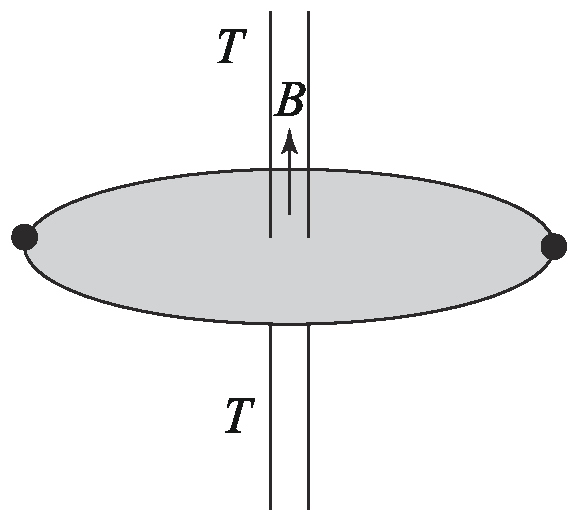
\includegraphics[width = 0.3\textwidth]{images/mag-18.pdf} 
\end{flushright}
\tagged{student}{\vspace*{0cm}}
\begin{taggedblock}{teacher}
\noindent
解析:电磁场自己的角动量。
\end{taggedblock}
\end{example}


\begin{example}
\textbf{【综合训练】}如图所示,一半径为$R$的轻质绝缘塑料薄圆盘水平放置,可绕过圆盘中心的竖直固定轴无摩擦地自由转动。
一半径为$a$的轻质小圆线圈($a\ll R$)固定在盘面上,圆线圈与圆盘共轴。
在盘边缘处等间隔地固定4个质量均为$m$的带正电的金属小球,每个小球所带电荷量均为$q$。
此装置处在一磁感应强度大小为$B_0$、方向竖直向上的均匀强磁场中,初始时圆盘静止,圆线圈中通有恒定电流$I$,
方向沿顺时针方向(从上往下看)。
若切断圆线圈中的电流,则圆盘将发生转动,求薄圆盘稳定转动后,圆盘在水平方向对每个金属球小的作用力的大小。

假设金属小球可视为质点,不计小圆线圈的自感和带电金属小球因运动所产生的磁场。
已知固定在圆盘面上的半径为$a$、通有电流$I$的圆线圈在圆盘面内、距线圈圆心的距离为$r$处($r\gg a$)产生的磁场的磁感应强度的大小为$B=k_m\frac{2\pi a^2 I}{r^3}$,式中$k_m$为已知常量,当线圈中的电流沿顺时针方向时,磁场方向垂直于圆盘平面且竖直向上.静电力常量为$k_e$。
\begin{flushright}
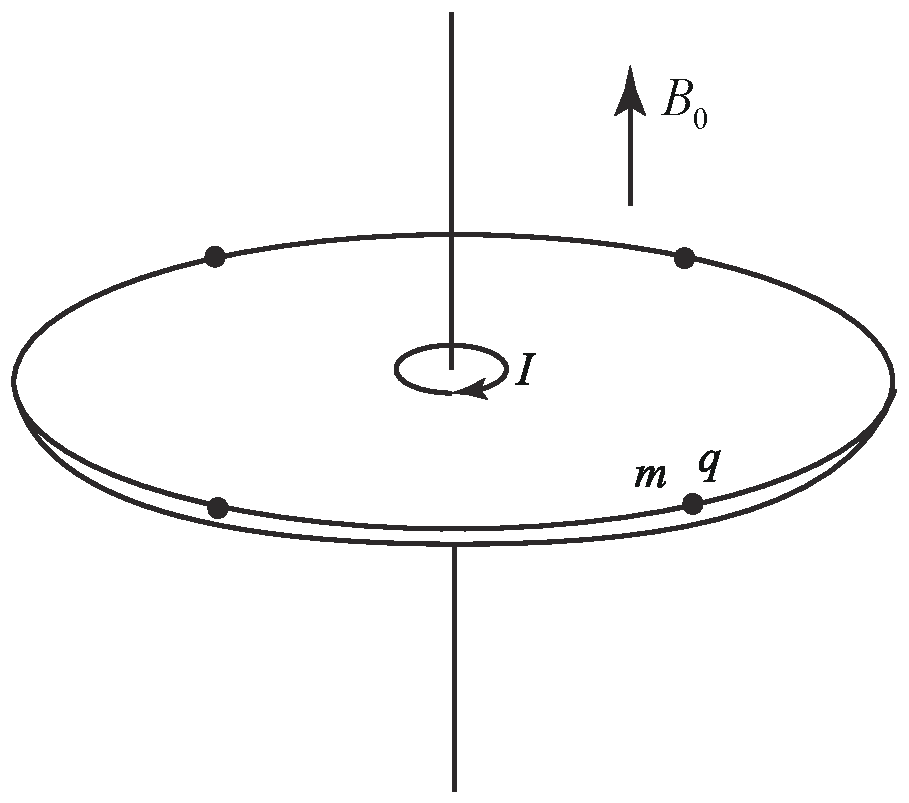
\includegraphics[width = 0.3\textwidth]{images/mag-19.pdf} 
\end{flushright}



\tagged{student}{\vspace*{6cm}}
\begin{taggedblock}{teacher}
\noindent
解析:$f=\frac{4k_m^2\pi^2a^4q^2}{mR^5}I^2+k_e\frac{q^2(1+2\sqrt{2})}{4R^2}-\frac{2k_m\pi a^2q^2B_0}{mR^2}I$
\end{taggedblock}
\end{example}


 \section{自感和互感}
 \subsection{自感现象、自感系数}

通过一个线圈的磁通量除了外加磁场以外,还包含有它自身产生磁场的贡献。
简单起见,假设外磁场为零,这样通过一个导体线圈内的磁通量完全由其自身所产生,当通过线圈的电流发生变化时,由它自身电流产生的磁场就会随之变化,这样通过线圈磁通量就会产生变化。
根据电磁感应定律,变化的磁通量会导致感生电动势,从楞次定律可知感生电动势必然会阻碍电流的变化,这个现象称为线圈的{\heiti 自感}(inductance),总的来说自感是导体自身电流变化产生的电磁感应现象。具有自感的线圈构成了一个电路元件,称为{\heiti 电感}(inductor)。
自感现象是导体的普遍性质,只是或大或小的区别,有时需要利用自感现象,有时自感会对电路造成破坏,需要尽量避免。

导体线圈的自感的大小由{\heiti 自感系数}(inductance)所给出,一般用$L$来代表,单位是$\mathrm{Henry}, \mathrm{H}, 1\mathrm{H} = 1 \Omega \cdot s$一个线圈的自感系数则是由线圈的形状、材料等一系列因素所决定,目前我们不需要从理论上对其进行计算。
对于一个线圈的自感系数为$L$的线圈,当它内部通有电流$I$时,通过线圈的磁通量
\begin{equation}
\Phi = LI,
\end{equation}
这样,当线圈当中的电流发生变化时自感产生的感应电动势\footnote{有时候线圈的形状也会发生变化,如果自感随线圈形状的关系为已知时自感电动势则由两部分组成:\[\mathcal{E} = -\frac{d\Phi}{dt} = -\frac{d}{dt}(LI) = -L\frac{dI}{dt}-\frac{dL}{dt}I.\]}
\begin{equation}
\mathcal{E} = -\frac{d\Phi}{dt} = -L\frac{dI}{dt},
\end{equation}
进一步可以得到当一个线圈内部通有电流$I$时,它所储存的磁能
\begin{equation}
E = \frac{1}{2}LI^2
\end{equation}


%%%%%%%%%%%%%%%%%%%%%%%%%%%%%%%%%%
\begin{example}
一个理想的密绕线圈(忽略边缘效应),截面为$S$,单位长度内绕有$n$匝线圈。
证明其自感系数$L = \frac{\mu_0 N^2 S}{l} = \mu n^2 V$,磁场能量密度为$\omega_M = \frac{B^2}{2\mu_0}$,其中$V$为线圈内的总体积。
\tagged{student}{\vspace*{4cm}}
\begin{taggedblock}{teacher}
\newline
解析:略
\end{taggedblock}
\end{example}
%%%%%%%%%%%%%%%%%%%%%%%%%%

%%%%%%%%%%%%%%%%%
\begin{example}

电磁驱动是与炮弹发射、航空母舰上飞机弹射起飞有关的一种新型驱动方式。
电磁驱动的原理如图所示,当直流电流突然加到一固定线圈上,可以将置于线圈上的环弹射出去。
现在同一个固定线圈上,先后置有分别用铜、铝和硅制成的形状、大小和横截面积均相同的三种环;当电流突然接通时,它们所受到的推力分别为$F_1$、$F_2$和$F_3$。
若环的重力可忽略,下列说法正确的是
\begin{flushright}
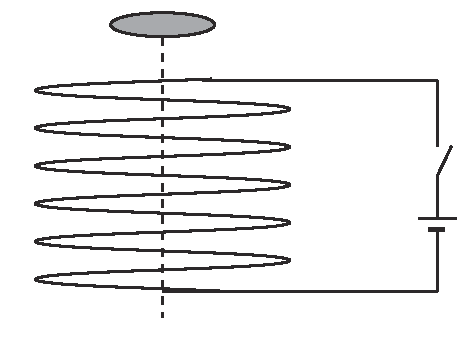
\includegraphics[width = 0.3\textwidth]{images/mag-28.pdf} 
\end{flushright}
\begin{eqnarray*}
 A. F_1>F_2>F_3\qquad  B. F_2>F_3>F_1\qquad C. F_3>F_2>F_1\qquad  D. F_1=F_2=F_3
\end{eqnarray*}
\tagged{student}{\vspace*{0cm}}
\begin{taggedblock}{teacher}
\noindent
解析:当线圈中通有电流时造成磁场的变化为给定,在不同的物质中由于其电阻的不同产生的感应电流也不尽相同,电阻越大电流越小,这样受到的安培力就越小。
从题目给出的物质来看,硅的电阻率最大,它的受力最小,虽然有可能不知道铜和铝的电阻率的大小,但选项中也只有$A$选项是合理的。

\end{taggedblock}
\end{example}
%%%%%%%%%%%%%%%%%%%%%%

%%%%%%%%%%%%%%%%%%%%%%%%%%%%%%%%%%
\begin{example}
如图所示的简单电路由一个自感为$L$的电感和一个阻值为$R$的电阻构成,$t=0$时回路中的电流为$I$,求此后回路中电流随时间的变化关系。
\begin{flushright}
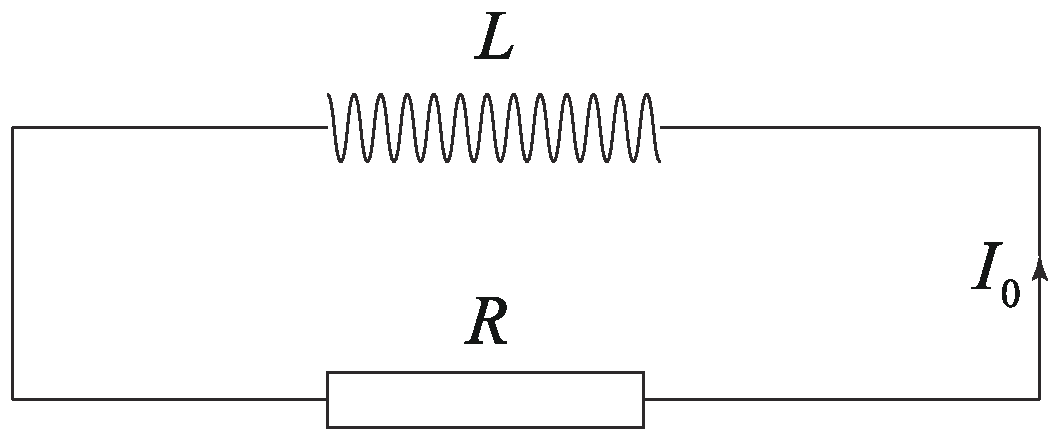
\includegraphics[width = 0.5\textwidth]{images/mag-39.pdf} 
\end{flushright}

\tagged{student}{\vspace*{4cm}}
\begin{taggedblock}{teacher}
\noindent
解析:由于电阻会消耗电能,会导致回路中电流的变化,当电流发生变化时电感并不是完全没有反应,而是会产生抵抗的电动势阻碍电流的变化。
在回路中电流变化满足的方程为
\[\mathcal{E} = -L \frac{dI}{dt} = IR,\qquad \frac{dI}{I} = - \frac{R}{L}dt,\]
求解微分方程可得:
\[
I(t) = I_0e^{- \frac{R}{L}t},
\]
可见$L$越大,电流衰减的速度就越慢,符合定性的认识。
\end{taggedblock}
\end{example}
%%%%%%%%%%%%%%%%%%%%%%%%%%


\begin{example}
一个中空的圆柱形的长度为$l$,内径为$r$,厚度为$d$,其中$l\gg r\gg d$,它由电阻率为$\rho$的材料制成。
有一个随时间变化的电流$I$从切向通过该柱体,假设电流在柱体长度方向上总是均匀分布。
并且柱体位置固定,不能够移动;简单起见在处理后面的问题中电流产生柱体外部的磁场忽略不计

\begin{center}
\includegraphics[width=0.6\textwidth]{images/3-2.pdf} 
\end{center}


\begin{enumerate}
\item 用通过柱体的电流、它的各种尺寸参数以及基本的物理常数写出其内部磁感应强度$B$。
\item 给出沿柱体圆周方向的感应电动势$\mathcal{E}$与通过电流随时间的变化率$\frac{dI}{dt}$、柱体的形状参数以及物理常数的关系式。
\item 给出感应电动势$\mathcal{E}$与电流$I$、电阻率$\rho$与柱体形状参数之间的关系。
\item 当$t=0$时的电流为$I_0$,求此后任意时刻$t>0$时的电流$I(t)$。
\end{enumerate}
\tagged{student}{\vspace*{4cm}}
\begin{taggedblock}{teacher}
\noindent
解析:$B=\frac{\mu_0 I}{l}$
\\$\mathcal{E}=-\frac{d(BS)}{dt}=-\frac{dB}{dt}S=-\frac{\mu_0\pi r^2}{l}\frac{dI}{dt}$
\\$\mathcal{E}=I*R=I*\frac{\rho ld}{2\pi r}$
\\$\frac{dI}{dt}+\frac{\rho l^2d}{2\pi r\mu_0 S}I=0$解出:$I=I_0*e^{-kt},k=\frac{\rho l^2d}{2\pi r\mu_0 S}$
\end{taggedblock}
\end{example}


%%%%%%%%%%%%%%%%%
\begin{example}
如图所示,有二平行金属导轨,相距$l$,位于同一水平面内(图中纸面),处在磁感应强度为$B$的匀强磁场中,磁场方向竖直向下(垂直纸面向里)。
质量均为$m$的两金属杆$ab$和$cd$放在导轨上,与导轨垂直。
初始时刻, 金属杆$ab$和$cd$分别位于$x = x_0$和$x =0$处。
假设导轨及金属杆的电阻都为零,由两金属杆与导轨构成的回路的自感系数为$L$。
今对金属杆$ab$施以沿导轨向右的瞬时冲量,使它获得初速$v_0$。
设导轨足够长,也足够大,在运动过程中,两金属杆之间距离的变化远小于两金属杆的初始间距$x_0$,因而可以认为在杆运动过程中由两金属杆与导轨构成的回路的自感系数$L$是恒定不变的。
杆与导轨之间摩擦可不计,求任意时刻两杆的位置$x_{ab}$和$x_{cd}$以及由两杆和导轨构成的回路中的电流$i$三者各自随时间$t$的变化关系。
\begin{flushright}
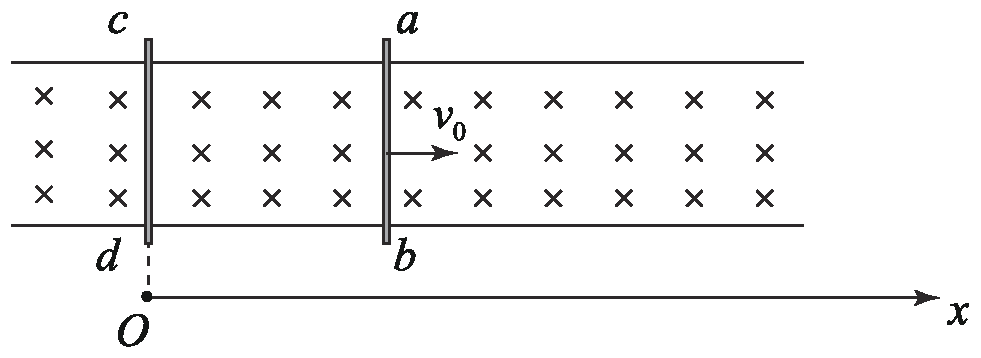
\includegraphics[width = 0.5\textwidth]{images/mag-22.pdf} 
\end{flushright}
\tagged{student}{\vspace*{4cm}}
\begin{taggedblock}{teacher}
\noindent
解析:$x_ab=x_0+\frac{1}{2}v_0t+\frac{v_0}{2Bl}\sqrt{\frac{mL}{2}}\sin(Bl\sqrt{\frac{2}{mL}})t$
\\$x_cd=\frac{1}{2}v_0t-\frac{v_0}{2Bl}\sqrt{\frac{mL}{2}}\sin(Bl\sqrt{\frac{2}{mL}})t$
\\$i=v_0\sqrt{\frac{m}{2L}}\sin(Bl\sqrt{\frac{2}{mL}})t$
\end{taggedblock}
\end{example}
%%%%%%%%%%%%%%%%%%%%%%




 \subsection{互感现象、互感系数}

当空间当中存在有两个线圈时,当其中一个线圈通电时,它所产生的磁感线有可能通过第二个线圈。
这样当第一个线圈的电流产生变化时,它会导致第二个线圈内的磁通量发生变化,而在第二个线圈当中产生感应电动势,这个现象称作线圈之间的互感应现象,简称{\heiti 互感}(mutual inductance)。
互感的大小用两个线圈之间的{\heiti 互感系数}(mutual inductance)$M$来表示,对于固定空间位置的两个线圈,当线圈1通有$I_1$的电流时,它的磁场通过线圈2的磁通量
\begin{equation}
\Phi_2 = M_{12}I_1,
\end{equation}
式中$M_{12}$称为线圈1对线圈2的互感系数。
同样的道理当线圈2通有电流$I_2$时它将在线圈1所围成的曲面上产生磁通
\begin{equation}
\Phi_1 = M_{21}I_2.
\end{equation}
任意两个线圈之间的互感系数之间必然有关系
\begin{equation}\label{eqn: 电磁感应-两个线圈的互感}
M_{12}=M_{21},
\end{equation}
它被两个线圈的位置、形状以及中间的材料所决定。
当线圈1当中的电流有变化时,它将会在线圈2当中产生感应电动势,其大小同样是由电磁感应定律给出:
\begin{equation}
\mathcal{E}_{12} = -M_{12}\frac{dI_1}{dt},
\end{equation}
同样地,当线圈2中电流随时间而变时也会在线圈1当中产生感应电动势,大小则正比于两者之间的互感系数和线圈2当中电流随时间的变化率。
当两个线圈分别通有电流$I_1$和$I_2$时,除了由于它们自身的自感所储存的磁能$\frac{1}{2}L_1I_1^2$和$\frac{1}{2}L_2I_2^2$以外,由于它们之间的互感,还将会有
\begin{equation}
E_{12}=M_{12}I_1I_2
\end{equation}
的磁能储存于两者之间。

\begin{example}
你能够证明关系式\ref{eqn: 电磁感应-两个线圈的互感}吗?
\tagged{student}{\vspace*{4cm}}
\begin{taggedblock}{teacher}
\newline
解析:假设它们不同,分别为$M_{12}$和$M_{21}$,那么我们对于两个线圈做如下的操作。
首先让线圈1通上$I_1$的电流,这时需要加入的能量$\frac{1}{2}L_1I_1^2$,然后让线圈2加上$I_2$的电流,这一步时除了要提供线圈2自感的能量以外,这个过程还会在线圈1上产生感应电动势。
因为那里已经有了电流,为了保证电流不变,需要外加克服感生电动势的功,这样总地算起来整个系统此时保存的能量就是
\[
\frac{1}{2}L_1I_1^2+\frac{1}{2}L_2I_2^2+M_{21}I_1I_2
\]
接下来我们首先让线圈1的电流变成零,为了维持线圈2内的电流不变需要外加电源作功,这一步可以取出$\frac{1}{2}L_1I_1^2+M_{12}I_1I_2$的能量,然后再使线圈2电流变成零,可以取出它的磁能,算总帐总共可以取出
\[
\frac{1}{2}L_1I_1^2+\frac{1}{2}L_2I_2^2+M_{12}I_1I_2
\]
的能量。
如果$M_{12}\neq M_{21}$必然能够通过这一手段取出能量而不产生其它变化,这是不允许的,所以两个线圈之间的互感系数必然相等。
\end{taggedblock}
\end{example}

%%%%%%%%%%%%%%%%%%%%%%%%%%%%%%%%%%
\begin{example}
求证,两个自感分别为$L_1$、$L_2$的线圈之间的互感系数$M_{12}^2 \le L_1L_2$,并给出等号成立的条件。
\tagged{student}{\vspace*{4cm}}
\begin{taggedblock}{teacher}
\newline
解析:当两个线圈分别通有$I_1$、$I_2$电流以后系统总能量
\begin{eqnarray*}
&&\frac{1}{2}L_1I_1^2+M_{12}I_1I_2+ \frac{1}{2}L_2I_2^2= \frac{1}{2}L_1\left(I_1+ \frac{M_{12}}{L_1}I_2\right)^2+\frac{1}{2}\left(L_2-\frac{M_{12}^2}{L_1}\right)I_2^2\ge 0
\end{eqnarray*}
第一项是平方必然大于等于零,在最不利的情况下它等于零,此时总能量大于零的条件就可以写成
\[M_{12}^2\le L_1L_2.\]
给出了互感系数的最大可能值。


\end{taggedblock}
\end{example}
%%%%%%%%%%%%%%%%%%%%%%%%%%



\begin{example}
大小线圈的半径分别为$a$和$b$,如图同轴放置,相距为$d$,满足$a\gg b$且$d\gg b$。
在小线圈中通入电流$I$,大线圈电阻$R$很大,所以不考虑感应电流的影响。
求电流均匀增加$( \frac{dI}{dt} = k)$时大线圈中的感应电流。
或电流不变,小线圈绕$z$轴以角速度$\omega$匀速转动(从上向下看是正方向),求大线圈中的感应电流。
\begin{flushright}
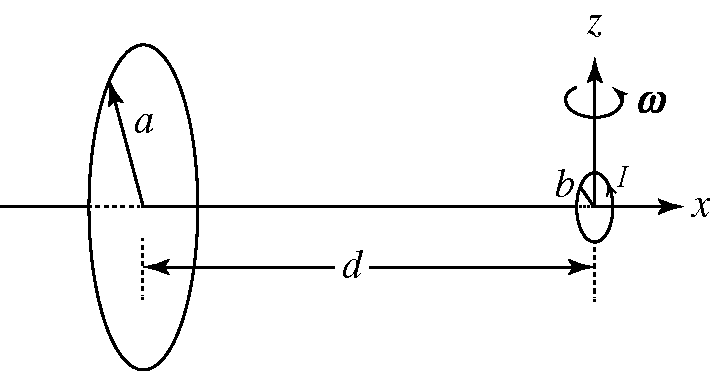
\includegraphics[width=0.5\textwidth]{images/mag-26.pdf}
\end{flushright}

\tagged{student}{\vspace*{4cm}}
\begin{taggedblock}{teacher}
\noindent
解析:$M_{21}=M_{12}$,需要计算小线圈对大线圈的互感系数,可以倒过来计算大线圈对小线圈的互感系数,若大线圈有电流I,则它在小线圈上产生电动势$\mathcal{E}=-M_{21}\frac{dI}{dt}$
\[M_{21}*\frac{dI}{dt}=\frac{d(BS)}{dt}=S*\frac{dB}{t}=\pi b^2\frac{dB}{dt}\]
由毕奥萨伐尔定律可得:\[B=\frac{\mu_0}{4\pi}\frac{I*2\pi a}{a^2+d^2}*\frac{a}{\sqrt{a^2+d^2}}\]
得出:
\[M_0=M_{12}=M_{21}=\frac{\mu_0\pi a^2b^2I}{2(a^2+d^2)^{\frac{3}{2}}}\]
感应电流\[I_1=\frac{M_0}{R}\frac{dI}{dt}=\frac{kM_0}{R}\]
若小线圈转动的话,S会变,所以M会改变
感应电流\[I_2=\frac{\mathcal{E}}{R}=\frac{d(BS)}{Rdt}=M_0\frac{d(I\cos\omega t)}{dt}=M_0*(\frac{dI}{dt}\cos\omega t-I\omega\sin\omega t)\]
\end{taggedblock}
\end{example}





 
\section{超导体的磁效应}
普通的导体有可能在某一特定温度之下电阻率突然降为零而形成{\heiti 超导体}(superconductor)。
除了电阻为零,超导体还有一个重要的性质--{\heiti 完全抗磁性}(perfect diamagnetism)或{\heiti 迈斯纳效应}(Meissner effect),指的是放置于磁场当中的超导体表面会产生感应电流,最终表面的感生电流产生的磁场与外磁场的叠加效应使得超导体内部的磁感应强度为零,称为超导体的完全抗磁性。
抗磁性产生的根源是处于超导状态的电子特有的性质。
超导体的这一性质有着很广泛的应用,著名的磁悬浮列车就是利用抗磁性而工作的,在近代大型粒子对撞机当中为了产生强磁场使高能粒子运行轨道偏转也需要借助超导体。
需要注意的是超导体只有当外磁场不是很强时才具有抗磁性,当外磁场的强度超过某一临界值时,就会破坏处于超导状态的电子对,使其失去抗磁性,超导体所能承受磁场的最大值称为它的{\heiti 临界磁场}(critical magnetic field)\footnote{ 除了临界温度和临界磁场以外,超导体所能够容纳的超导电流也不能无限地增加,当通过超导体的电流超过临界电流时也会失去超导电性}。
导线回路中的超导体可以看成是理想的导线,它可以没有电阻,但是一般要考虑回路的电感,在超导体两段加电动势的结果是使得回路里的电流发生改变。


\begin{example}
为了判断一个导体是否处于超导态,可以在其内部通一定的电流,如果超导体内的电流永不消失则可判定为超导体。

为此目的用直径为$1\unit{mm}$的超导材料制成的导线做成一个半径为$5\unit{cm}$的圆环,圆环处于超导态。
环内通有$100\unit{A}$的电流,一年以后发现圆环内电流变化量小于$10^{-6}\unit{A}$。
试估计此超导材料电阻率数量级的上限。

已知半径为$r$的圆环中通一电流$I$后,圆环中心的磁感应强度$B = \frac{\mu_0 I}{2r}$,式中各量均用国际单位,$\mu_0 = 4\pi\pow{-7}\unit{NA^{-2}}$。
\tagged{student}{\vspace*{4cm}}
\begin{taggedblock}{teacher}
\newline
解析:$7.5*10^{-29}\Omega*m$
\end{taggedblock}
\end{example}

\begin{example}
可以利用超导线圈寻找{\heiti 磁单极子},和条形磁铁同时具有南、北极不同的是磁单极子带有非零的磁荷。
试分析当一个磁单极子从超导线圈中间穿过以后会发生的现象。
\begin{flushright}
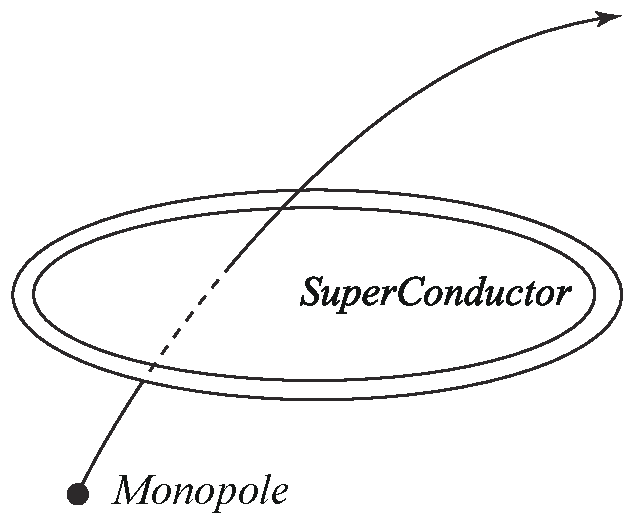
\includegraphics[width = 0.4\textwidth]{images/mag-41.pdf} 
\end{flushright}
\tagged{student}{\vspace*{0cm}}
\begin{taggedblock}{teacher}
\noindent
解析:当磁单极穿过超导线圈之后,由于磁通量发生了变化,会在超导体中留下感应电流,而此感应电流由于超导电性很长时间不会消失。
放置一个原先没有电流的超导线圈,一段时间以后测量它内部的电流,如果有电了说明有磁单极穿过。
人们就是用这种方法寻找磁单极,但至令还没有找到。
\end{taggedblock}
\end{example}

\begin{example}
图中$oxy$是位于水平光滑桌面上的直角坐标系,在$x>0$的一侧,存在匀强磁场,磁场方向垂直于$oxy$平面向里,磁感应强度的大小为$B$。
在$x<0$的一侧,一边长分别为$l_1$和$l_2$的刚性矩形超导线框位于桌面上,框内无电流,框的一对边与$x$轴平行。
线框的质量为$m$,自感为$L$,现让超导线框沿$x$轴方向以初速度$v_0$进入磁场区域,试定量地讨论线框以后可能发生的运动情况及与初速度大小的关系。(假定线框在运动过程中始终保持超导状态)
\begin{flushright}
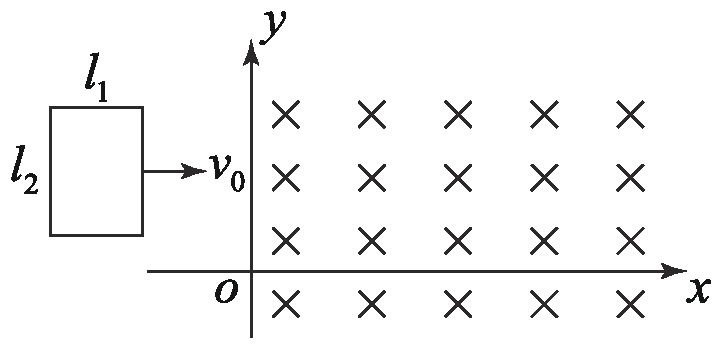
\includegraphics[width = 0.5\textwidth]{images/mag-24.pdf} 
\end{flushright}
\tagged{student}{\vspace*{4cm}}
\begin{taggedblock}{teacher}
\noindent
解析:
\\1.初速度\[v_0\le\frac{Bl_1l_2}{\sqrt{mL}}\]
在安培力作用下,为半个周期的简谐振动。
\\振动方程为:\[x=\frac{v_0\sqrt{mL}}{Bl_2}\sin(\frac{Bl_2}{\sqrt{mL}}t)\]
经过时间\[t=\frac{T}{2}=\pi\frac{\sqrt{mL}}{Bl_2}\]后,线框退出磁场,以速度$v_0$向左匀速运动。
\\2.初速度较大:\[v_0\ge\frac{Bl_1l_2}{\sqrt{mL}}\]
在安培力作用下,做不到四分之一个周期的简谐运动,
\[t_1=\frac{\sqrt{mL}}{Bl_2}\arcsin\frac{Bl_1l_2}{\sqrt{mLv_0^2}}\]
最后向右匀速前进\[v=\sqrt{v_0^2-\frac{B^2l_1^2l_2^2}{mL}}\]。
\end{taggedblock}
\end{example}


%%%%%%%%%%%%%%%%%%%%%%%%%%%%%%%%%%
\begin{example}
磁悬浮列车是一种高速运载工具,它具有两个重要系统。
一是悬浮系统,利用磁力(可由超导电磁铁提供)使车体在导轨上悬浮起来与轨道脱离接触。
另一是驱动系统,在沿轨道上安装的三相绕组(线圈)中,通上三相交流电,产生随时间、空间作周期性变化的磁场,磁场与固连在车体下端的感应金属板相互作用,使车体获得牵引力。

为了有助于了解磁悬浮列车的牵引力的来由,我们求解下面的问题。
设有一与轨道平面垂直的磁场,磁感应强度$B$随时间$t$和空间位置$x$变化规律为
\[B(x,t) = B_0\cos(\omega t-kx),\]  
式中$B_0、\omega 、 k$均为已知常量,坐标轴$x$与轨道平行。
在任一时刻$t$,轨道平面上磁场沿$x$方向的分布是不均匀的,如图所示。
图中$Oxy$平面代表轨道平面,×表示磁场的方向垂直$Oxy$平面指向纸里,$\cdot$ 表示磁场的方向垂直$Oxy$平面指向纸外。
规定指向纸外时B取正值,×和$\cdot$的疏密程度表示沿着$x$轴$B$的大小分布。
一与轨道平面平行的具有一定质量的金属矩形框$MNPQ$处在该磁场中,已知与轨道垂直的金属框边$MN$的长度为$l$,与轨道平行的金属框边$MQ$的长度为$d$,金属框的电阻为$R$,不计金属框的电感。

1.试求在时刻$t$,当金属框的$MN$边位于$x$处时磁场作用于金属框的安培力,设此时刻金属框沿$x$轴正方向移动的速度为$v$。 

 2.试讨论安培力的大小与金属框几何尺寸的关系。 
 \begin{flushright}
 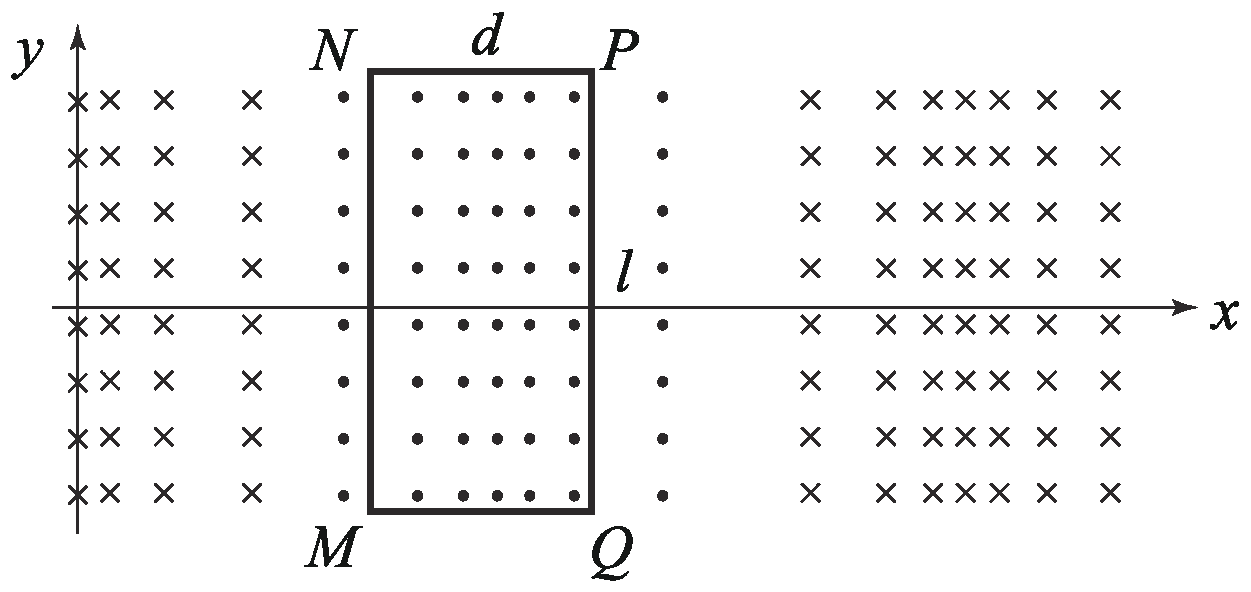
\includegraphics[width = 0.6\textwidth]{images/mag-40.pdf} 
 \end{flushright}

\tagged{student}{\vspace*{4cm}}
\begin{taggedblock}{teacher}
\noindent
解析:
\\1.\[F=\frac{4B_0^2l^2(\frac{\omega}{k}-v)}{R}\sin^2(\frac{kd}{2})\]
2.当$d=\frac{2n\pi}{k},n=1,2,3,...$
\[F=0\]
当$d=\frac{(2n+1)\pi}{k},n=1,2,3,...$,此时F达到最大值
\[F=F_{max}=\frac{4B_0^2l^2(\frac{\omega}{k}-v)}{R}\]
当d取其它值时,F介于0与最大值之间。
\end{taggedblock}
\end{example}
%%%%%%%%%%%%%%%%%%%%%%%%%%

